\chapter{提案手法}
既存手法のgBoostでは探索木上を深さ優先的に厳密探索する.
しかし,入力グラフ集合に対して,個々のグラフの大きさや全体数の増加に伴い,
存在しうる部分グラフの総数は組合せ的に増加するため,厳密探索におけるコストは莫大なものである.
問題によってモデル構築が困難なものも存在する.
したがって,本稿では,厳密探索ではなく,確率的に探索を行う手法を提案する.

\section{探索空間}
既存手法では,探索空間としてgSpan\cite{gSpan}のDFSコード木を利用していたが,
提案手法では,DFSコード木から同型判定を除外した探索空間を用いる.
つまり,提案手法では,同じ部分グラフを表すノードが複数箇所に出現することを許容した,
DFSコード木を拡大した探索木を利用し,特徴探索を行う.
この探索空間の変更の詳細は\ref{search space}において言及する.

\section{確率的探索}
まず初めに,本提案手法で用いる探索パスおよび$K$パス探索を定義する.
\begin{Definition}[探索パス]
	根ノードを始点とし,子ノードを列挙する.列挙した子ノードの中からある確率分布$P$に従い一つの子ノードを選択する.
	子ノードの列挙,選択の動作を葉ノードに達するまで繰り返す.
	以上の動作によって選択された根ノードから葉ノードまでのパスを探索パスと定義する.
\end{Definition}
\begin{Definition}[$K$パス探索]
	$K$本の探索パスによってカバーされるノード集合における特徴探索を$K$パス探索と定義する.
\end{Definition}

以下では$K$パス探索を用いた,提案手法の枠組みを説明する.
Algorithm\ref{alg_main}に探索アルゴリズムの擬似コードを示す.ここでは探索木のノード$x$と対応する部分グラフを同一視する.
%アルゴリズムがここに入る
\begin{algorithm}
	\small 
	\caption{確率的特徴探索}\label{alg_main}
	\begin{algorithmic}[1]
		\Procedure{RandomSearch}{k}
		\State グローバル変数 : $t^*,\omega^*,g^*$
		%		\State 最適な部分グラフ$t^*,\omega^*$を探索
		\State $x \gets \text{根ノード}$ 
		\State \textsc{Grow}($x,K$)
		\EndProcedure

		\Function{Grow}{$x,K$}
		\State $x$に対するgain $g(x)$, bound $b(x)$を計算
		\If {$b(x) < g^*$}
		\State \textbf{return}
		\EndIf
		\If {$g^* < g(x)$}
		\State $t^* \gets x,\omega^* \gets \omega,g^* \gets g(x)$
		\EndIf
		\If {$x$が葉ノード}
		\State \textbf{return}
		\EndIf
		\State$C$ = \{$x$の子ノード\}
		\State 集合$C$上の確率分布$P$を計算 \Comment{提案手法1〜3}
		\State $\{k_c\} \gets \textsc{SampleCount}(C,K,P)$
		\ForAll{$c \in C$}
		\If {$k_c > 0$}
		\State \textsc{Grow}($c,k_c$)
		\EndIf
		\EndFor
		\EndFunction

		\Function{SampleCount}{$C,K,P$}
		\State $k_c \gets 0$ for all $c \in C$ \Comment{子ノード$c$の選択回数を保存}
		\For{$i=1$ to $K$}
		\State $c \gets \text{$P$に基づき子ノード一つをサンプリング} $
		\State $k_c \gets k_c + 1$
		\EndFor
		\State \textbf{return} $\{k_c\}$
		\EndFunction
	\end{algorithmic}
\end{algorithm}

%アルゴリズムの説明がここに入る
Algorithm\ref{alg_main}では,$K$パス探索において同一ノードの探索を複数回行わないために,探索とパスの成長を同時に行う.
まず,根ノードを始点に設定し,探索パスの本数$K$とともに\textsc{Grow}関数へ渡す.
\textsc{Grow}関数では引数として渡されたノードにおけるgainとboundの値を式\eqref{eq:gain}および\eqref{eq:bound}で計算(探索)し,既存手法と同様にしてboundの値で探索の枝刈りを行う.
gainの値がこれまでの最良値である場合には保存する.
その後,渡されたノードが葉ノードではない場合には子ノードを列挙し($C$),列挙した子ノード集合上に選択確率分布$P$を設定する.
\textsc{SampleCount}関数内で,設定した確率分布$P$に基づきサンプリングを行い, $K$を各子ノードに割り振る.
各子ノード$c$に対応する整数$k_c$が$0$より大きい場合,\textsc{Grow}関数にそれぞれを引渡し再帰的に探索を行う.
以上のアルゴリズムにより深さ優先的な$K$パス探索を達成する.

本研究では探索手順における,子ノードの選択確率分布$P$に関して,以下に示す3つの確率設定手法を提案する.

\subsection{提案手法1:一様確率設定}
提案手法1では,子ノードに対して一様に確率を設定する.
現探索ノードの子ノード集合を$C$とすると,
子ノード$c$の選択確率を以下に示す.
\[
	P(c) = 1 / |C|.
\]

\subsection{提案手法2:支持度(support)の情報を加えた確率設定}
提案手法1は,入力グラフの特徴を利用しないナイーブな手法である.
本節では,入力グラフに対する支持度(support)の情報を利用した手法を提案する.
ある部分グラフ$x \in \mathcal{T}$の支持度とは,$x$が$\ell$個の全入力グラフの内いくつのグラフで現れるかを表す値であり以下の式で定義される.
\[
	\sigma(x) = \sum_{n=1}^{\ell} \mathbb{I} (x \subseteq G_n) .
\]
$\ell$は入力グラフの総数,$\mathcal{T}$は入力グラフにおける部分グラフ集合である.

探索木の性質上,支持度が大きい部分グラフのほうが小さいものに比べて
複数の入力グラフ上での拡大グラフを考えることができるため,子孫空間が広いことを期待できる.
子孫空間が狭いノードに多くの探索パスを伸ばす場合,探索が広がらず無駄になる可能性が大きい.
したがって,本手法では支持度が大きい子ノードが選択されやすくなるよう確率を定める.
現探索ノードの子ノード集合を$C$とすると,
子ノード$c$の選択確率を以下に示す.
\[
	P(c) = \sigma(c) / \sum_{t \in C} \sigma(t).
\]

\subsection{提案手法3:boundの情報を加えた確率設定}
本節では,式\eqref{eq:bound}のbound $b(t)$の情報を利用した手法を提案する.
$b(t)$は$t$の子孫ノードで得ることのできるgainの上限値を表すため,
boundの大きな子ノードへの探索を行うことで,より大きなgainの値を得ることが期待できる.
したがって,本手法ではboundの値が大きい子ノードが選択されやすくなるよう確率を定める.
現探索ノードの子ノード集合を$C$とすると,
子ノード$c$の選択確率を以下に示す.
\[
	P(c)  =  b(c) / \sum_{t \in C} b(t).
\]

本手法はboundの値を用いるため,予め全ての子ノードを探索する必要がある.
したがって,提案手法1,2に比べて1本の探索パスを伸ばすときの探索ノード数が多くなることが予想される.

\section{探索空間の同型判定除外}
\label{search space}
既存手法では,gSpan\cite{gSpan}アルゴリズムで構築されるDFSコード木を探索空間として用いている.
gSpanアルゴリズムでは,グラフ同型問題を解き,
同型である場合には当アルゴリズムで定義される辞書順を用いて最小のものだけを木に採用する.
つまり,辞書順最小でないノードが現れた際には,そのノードを木に含まない.

ここで問題となるのが,DFSコード木に探索パスを流す際,
探索パスが辞書順最小ではないノードに向かうと途中でパスの成長が止まってしまうという点である.
このようなパスの滞りが多く発生する場合,下層のノード、つまり大きな部分グラフを表すノードの探索をうまく行うことが出来ない.

したがって本研究では,gSpanアルゴリズムでのグラフ同型判定を行わずに,
辞書順最小でないノードも木に追加することで,
探索パスの滞りを防ぎ,各階層での探索に偏りが生じないよう探索空間を変更する.

\chapter{実験と結果}
\section{データセット}
\begin{table}
	\centering
	\begin{tabular}{|c|r|r|r|r|r|}
		\hline
		データ名 & グラフ数 & 平均ノード数 & 平均エッジ数 & 正例 & 負例\\
		\hline \hline
		CPDB  & 684 & 25.2 & 25.6 & 341 & 343\\
		\hline
		Mutag & 188 & 26.3 & 28.1 & 125 & 63\\
		\hline
	\end{tabular}
	\caption{使用したデータセット}
	\label{dataset}
\end{table}

本稿では,gBoostの元論文\cite{gBoost}で用いられた化合物データセットのうち2つを使用した.
ただし,元論文\cite{gBoost}と異なり,化合物のグラフ表現は,水素を明示的に付与し,Sybyl Mol2形式で頂点ラベル,辺ラベルを付与した分子グラフである.\ref{dataset}に各データセットのグラフ数,平均ノード・エッジ数,正例と負例の数を示す.

\section{実験1:探索の精度,効率に関する実験}
実験1では,CPDBデータに対して各提案手法がどれだけ精度よく探索できているか,
どれだけ既存手法より効率化できているかを計る実験を行う.
本稿では,式\eqref{eq:dualprob}の双対問題における目的関数の最終値を探索精度の指標に,
モデル構築までにgainとboundの値を計算したノードの総数を探索ノード数とし,効率化の指標に用いる.
以下では,誤分類に対するコスト制御のパラメータ$\nu$の値が0.1,0.3,0.5の3つの場合に対して実験を行う.
(その他のパラメータ設定に関しては,gBoostにおける固定値maxpat=10,$\epsilon$=0.01を用いる.)

初めに,探索パスの本数パラメータ$K$を変化させた時の目的関数の最終値の推移を図\ref{1-1}に示す.
横軸は$K$,縦軸は目的関数の最終値である.$K$の刻み幅は,提案手法1,2に対しては10とする.
提案手法3は,アルゴリズム上,子ノードのgainとboundを全て計算する必要があるため,
提案手法1,2と比べて探索ノード数が多くなる.したがって,$K$の刻み幅は1とする.
\begin{figure*}[t]
	\begin{center}
		\begin{tabular}{c}
			\begin{minipage}{0.33\hsize}
				\begin{center}
					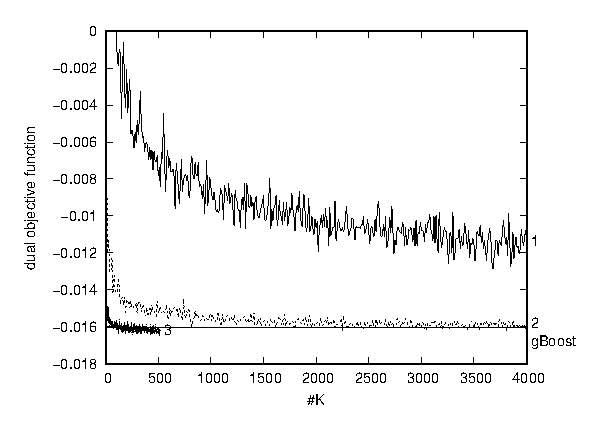
\includegraphics[width=55mm]{cpdb/purpose_1.eps}
				\end{center}
				\vspace{0.5cm}
				\subcaption{$\nu = 0.1$}
				\label{fig:1}
			\end{minipage}
			\begin{minipage}{0.33\hsize}
				\begin{center}
					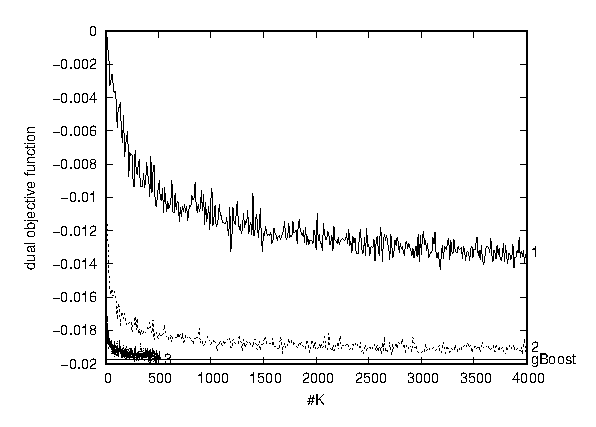
\includegraphics[width=55mm]{cpdb/purpose_3.eps}
				\end{center}
				\vspace{0.5cm}
				\subcaption{$\nu = 0.3$}
				\label{fig:2}
			\end{minipage}
			\begin{minipage}{0.33\hsize}
				\begin{center}
					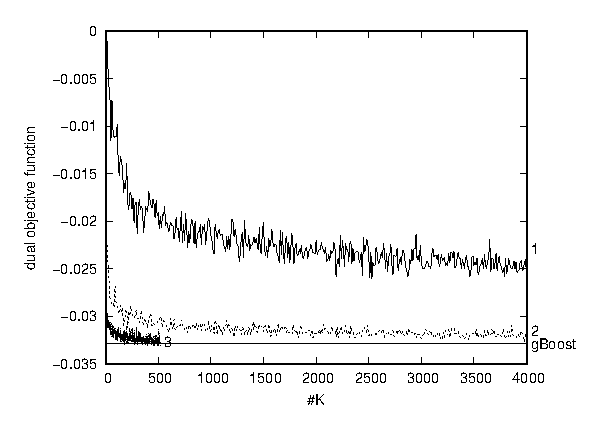
\includegraphics[width=55mm]{cpdb/purpose_5.eps}
				\end{center}
				\vspace{0.5cm}
				\subcaption{$\nu = 0.5$}
				\label{fig:3}
			\end{minipage}
		\end{tabular}
		\caption{実験1-1(K - 目的関数)}
		\label{1-1}
	\end{center}
\end{figure*}

次に,$K$の数を変化させた時の探索ノード数の推移を図\ref{1-2}に示す.
横軸は$K$,縦軸は探索ノード数である.
$K$の刻み幅は,前述したものと同じ値とする.
\begin{figure*}[t]
	\begin{center}
		\begin{tabular}{c}
			\begin{minipage}{0.33\hsize}
				\begin{center}
					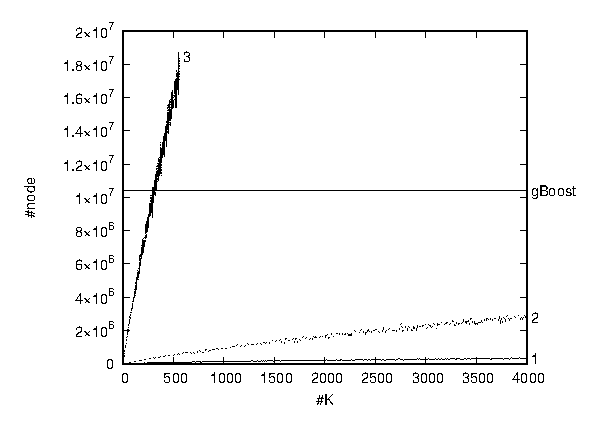
\includegraphics[width=55mm]{cpdb/node_1.eps}
				\end{center}
				\vspace{0.5cm}
				\subcaption{$\nu = 0.1$}
				\label{fig:4}
			\end{minipage}
			\begin{minipage}{0.33\hsize}
				\begin{center}
					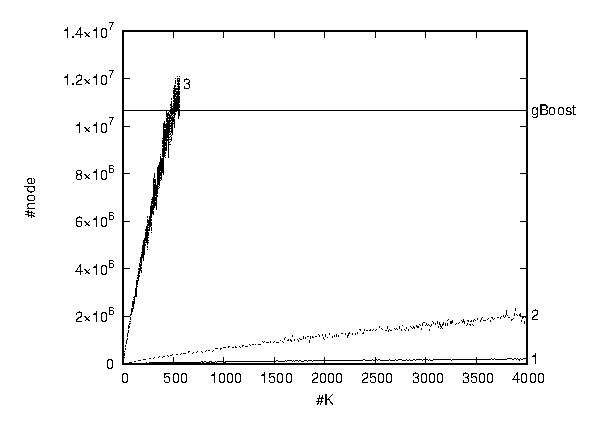
\includegraphics[width=55mm]{cpdb/node_3.eps}
				\end{center}
				\vspace{0.5cm}
				\subcaption{$\nu = 0.3$}
				\label{fig:5}
			\end{minipage}
			\begin{minipage}{0.33\hsize}
				\begin{center}
					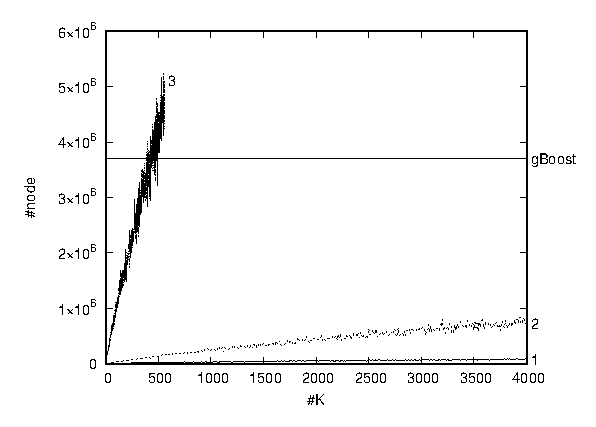
\includegraphics[width=55mm]{cpdb/node_5.eps}
				\end{center}
				\vspace{0.5cm}
				\subcaption{$\nu = 0.5$}
				\label{fig:6}
			\end{minipage}
		\end{tabular}
		\caption{実験1-2(K - 探索ノード数)}
		\label{1-2}
	\end{center}
\end{figure*}

最後に,前述した2つの実験から,各提案手法の探索ノード数に対して,目的関数の最終値の推移を図\ref{1-3}に示す.
横軸は探索ノード数,縦軸は目的関数の最終値である.
\begin{figure*}[t]
	\begin{center}
		\begin{tabular}{c}
			\begin{minipage}{0.33\hsize}
				\begin{center}
					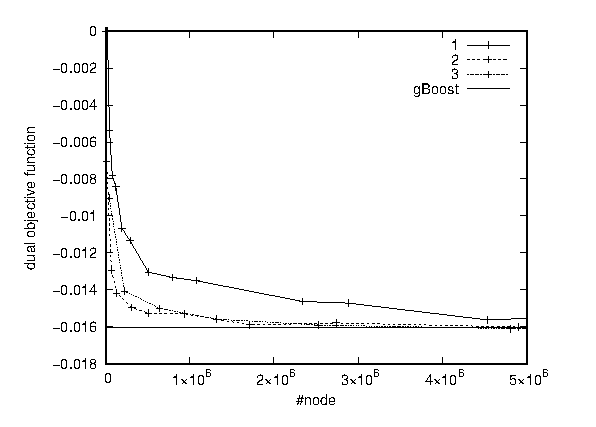
\includegraphics[width=55mm]{cpdb/purpose_node_1.eps}
				\end{center}
				\vspace{0.5cm}
				\subcaption{$\nu = 0.1$}
				\label{fig:7}
			\end{minipage}
			\begin{minipage}{0.33\hsize}
				\begin{center}
					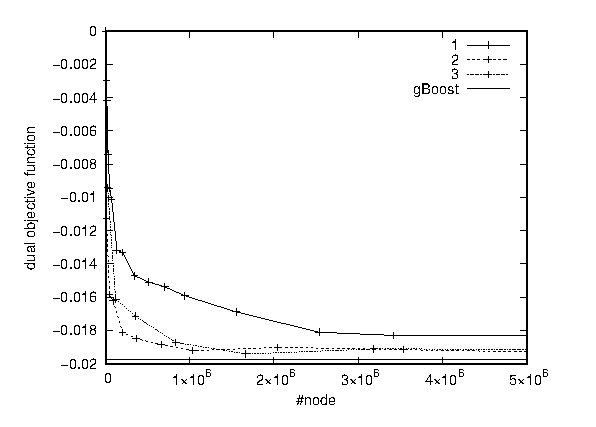
\includegraphics[width=55mm]{cpdb/purpose_node_3.eps}
				\end{center}
				\vspace{0.5cm}
				\subcaption{$\nu = 0.3$}
				\label{fig:8}
			\end{minipage}
			\begin{minipage}{0.33\hsize}
				\begin{center}
					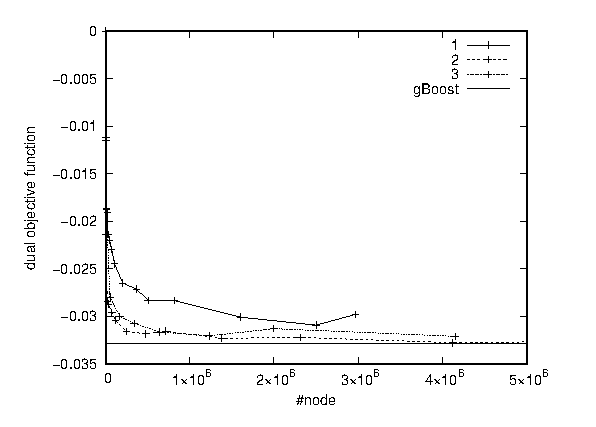
\includegraphics[width=55mm]{cpdb/purpose_node_5.eps}
				\end{center}
				\vspace{0.5cm}
				\subcaption{$\nu = 0.5$}
				\label{fig:9}
			\end{minipage}
		\end{tabular}
		\caption{実験1-3(探索ノード数 - 目的関数)}
		\label{1-3}
	\end{center}
\end{figure*}

\section{実験2:乱数の影響に関する実験}
提案手法では,乱数を使用しているため,結果に分散が生じる.
したがって,実験2ではCPDBデータに対して各提案手法が乱数にどれだけ影響を受けるのかを調べる.
$K$の数を10,100,1000とし,乱数に10個のシード値を与えた時の各提案手法での目的関数の最終値の平均,分散,探索ノード数の平均値を比較する.
$\nu$の値を0.3に固定し,
表\ref{randomseed}に結果を示す.
\begin{table}[t]
	\centering
	\begin{tabular}{|c|r|r|r|r|r|}
		\hline
		K 10 & 目的関数平均 & 分散 & 探索ノード数平均 \\
		\hline \hline
		提案手法1  & 0 & 0 & 1625.0 \\
		\hline
		提案手法2  & -0.011543 & 3.0385e-04 & 9000.8 \\
		\hline
		提案手法3  & -0.017377 & 1.7890e-04 & 277280.6 \\
		\hline
		\hline
		K 100 & 目的関数平均 & 分散 & 探索ノード数平均 \\
		\hline \hline
		提案手法1  & -0.004994 & 2.6913e-04 & 16253.6 \\
		\hline
		提案手法2  & -0.016711 & 9.4498e-05 & 86857.9 \\
		\hline
		提案手法3  & -0.019121 & 6.4197e-05 & 2456806.0 \\
		\hline
		\hline
		K 1000 & 目的関数平均 & 分散 & 探索ノード数平均 \\
		\hline \hline
		提案手法1  & -0.011567 & 2.8003e-04 & 84839.9 \\
		\hline
		提案手法2  & -0.018501 & 8.2502e-05 & 647241.9 \\
		\hline
		提案手法3  & -0.019604 & 6.2834e-05 & 19284961.9 \\
		\hline
	\end{tabular}
	\caption{実験2}
	\label{randomseed}
\end{table}

\section{実験3:モデルの予測精度に関する実験}
実験3では,既存手法と3つの提案手法を用いて構築された予測モデルの実際の予測精度を比較する.
データにはCPDB,Mutagの2つのデータを利用する.
既存手法の精度が10分割交差検証の正答率の値で測られるため,
各提案手法では10分割交差検証を10回行い,正答率の平均値,分散値,
探索ノード数の平均値を求め,各手法の精度を比較する.
$\nu$の値が,0.01,0.1,0.2,0.3,0.4,0.5,0.6の場合に対して実験を行なう.
\begin{figure*}[t]
	\begin{minipage}{0.5\hsize}
		\begin{center}
			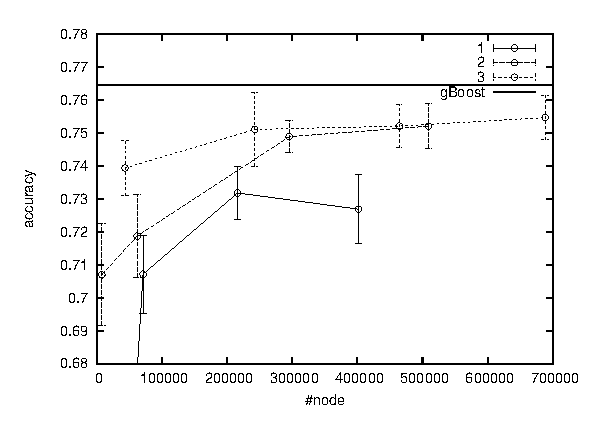
\includegraphics[width=65mm]{cpdb/node_acc.eps}
		\end{center}
		\vspace{0.5cm}
		\subcaption{gBoostの最良$\nu$パラメータを用いた場合}
		\label{fig:10}
	\end{minipage}
	\begin{minipage}{0.5\hsize}
		\begin{center}
			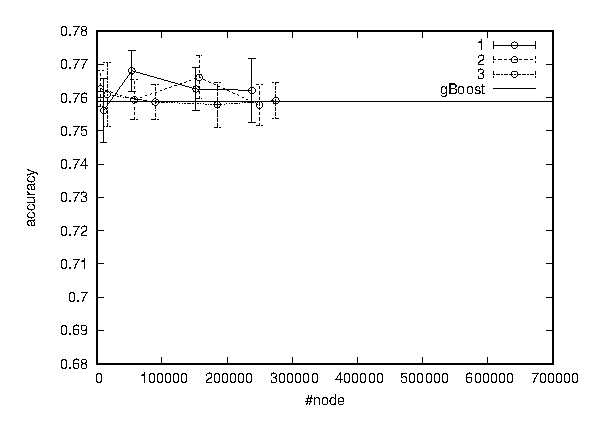
\includegraphics[width=65mm]{cpdb/node_acc_para.eps}
		\end{center}
		\vspace{0.5cm}
		\subcaption{各手法で$\nu$パラメータのチューニングを行なった場合}
		\label{fig:11}
	\end{minipage}
	\caption{実験3(探索ノード数 - 正答率)CPDB}
	\label{cpdb_acc}
\end{figure*}
\begin{figure*}[t]
	\begin{minipage}{0.5\hsize}
		\begin{center}
			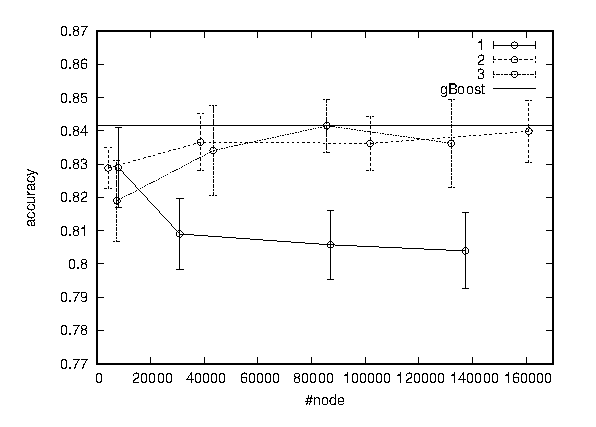
\includegraphics[width=65mm]{mutag/node_acc.eps}
		\end{center}
		\vspace{0.5cm}
		\subcaption{gBoostの最良$\nu$パラメータを用いた場合}
		\label{fig:12}
	\end{minipage}
	\begin{minipage}{0.5\hsize}
		\begin{center}
			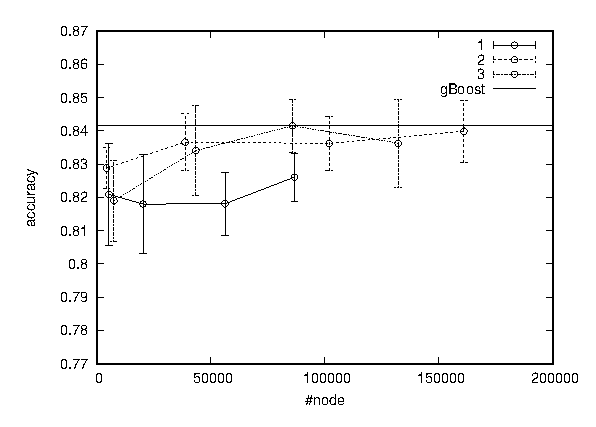
\includegraphics[width=65mm]{mutag/node_acc_para.eps}
		\end{center}
		\vspace{0.5cm}
		\subcaption{各手法で$\nu$パラメータのチューニングを行なった場合}
		\label{fig:13}
	\end{minipage}
	\caption{実験3(探索ノード数 - 正答率)Mutag}
	\label{mutag_acc}
\end{figure*}
横軸を探索ノード数,縦軸を正答率の値とし,図\ref{cpdb_acc},図\ref{mutag_acc}に結果を示す.

\section{実験4:探索空間の変更に関する実験}
提案手法では,各階層での探索の偏りを防ぐために,既存手法で利用する探索木を拡大した探索木を用いている.
実験4ではCPDBデータに対して,探索木を変更したことによる探索精度の影響を調べる.
$\nu$の値を0.3に固定し,探索ノード数に対する目的関数の結果を,
数既存手法で用いる探索木を利用した場合と,提案手法で変更した探索木を利用した場合とで比較する.
\begin{figure*}[t]
	\begin{minipage}{0.5\hsize}
		\begin{center}
			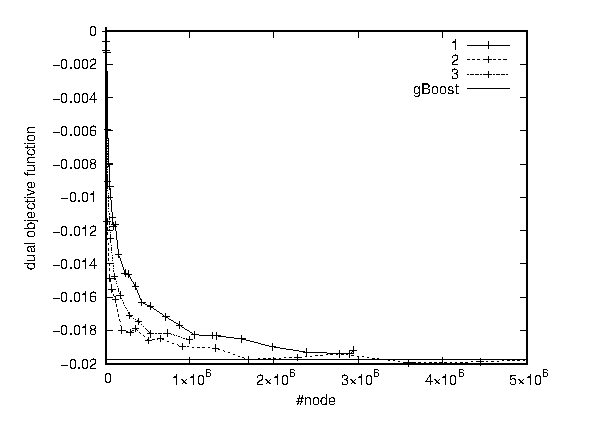
\includegraphics[width=55mm]{cpdb/purpose_node_3_tree.eps}
		\end{center}
		\vspace{0.5cm}
		\subcaption{既存の探索木(DFSコード木)を用いた場合}
		\label{fig:14}
	\end{minipage}
	\begin{minipage}{0.5\hsize}
		\begin{center}
			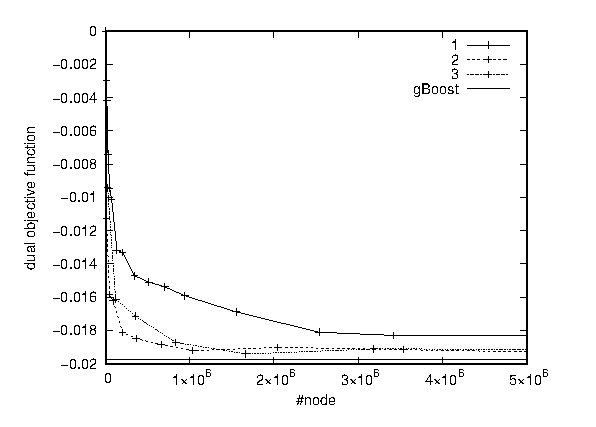
\includegraphics[width=55mm]{cpdb/purpose_node_3.eps}
		\end{center}
		\vspace{0.5cm}
		\subcaption{変更した探索木を用いた場合}
		\label{fig:15}
	\end{minipage}
	\caption{実験4 探索木の変更による影響}
	\label{tree}
\end{figure*}
横軸を探索ノード数,縦軸を目的関数の最終値とし,図\ref{tree}に結果を示す.

\chapter{考察}
\label{考察}
\section{実験1}
図\ref{1-1}から見て取れるように,同数の探索パスを伸ばす場合には,提案手法3,2,1の順に目的関数の値が良い値となった.
この理由としては,図\ref{1-2}のように,
ランダムに探索パスを伸ばすよりもグラフの特徴を利用した方が広く探索を行えるからであると考えられる.
図\ref{1-2}において,提案手法3のノード数が他の手法より莫大に多くなるのは,
前述したとおり子ノードのboundを利用して確率を振るためには予め全ての子ノードを探索する必要があるためである.
また,手法3が既存手法の探索ノード数を上回る理由としては,
既存手法の探索木から同型判定を除外したため,既存手法よりも探索空間が広くなっているためであると考えられる.

次に各提案手法の優位性を図\ref{1-3}より考える.
探索の効率として,探索ノード数に応じた目的関数の最終値を考えると,
提案手法1が他と比べて少し劣る結果となった.
これには2つの理由が予想される.
1つ目は,提案手法1は,2と3に比べて探索パスに対する探索ノード数が少ない(図\ref{1-2}).
したがって,他の手法と同程度のノード数を探索するためには,探索パスの数を増やす必要がある.
ここで問題であるのが,本探索空間は同型判定を除外しているため,
同じ部分グラフを表現するノードが複数存在しうることである.
探索パスの数が多い時は少ない時に比べて,この同じ部分グラフを表現する異なるノードにたどり着く確率が大きくなる.
これらのノードは子孫の空間が同じであるため,探索が無駄になる可能性が生じる.
したがって,同探索ノード数での目的関数の値が他の手法より劣る結果になったのではないかと予想される.
2つ目は,提案手法2,3に関しては,グラフの特徴を利用した探索手法であるのに対し,
提案手法1ではグラフの特徴を利用しないナイーブな手法であるという点が挙げられる.
この点より,提案手法1の探索空間よりも,他2つの探索空間のほうが
目的関数に寄与する特徴を含みやすいのではないかと考えられる.
以上の2つの理由から,提案手法1が他の手法より劣る結果となったと考る.
提案手法2と3に関しては,同程度の探索効率であることが見て取れる.

\section{実験2}
探索ノード数を基準として分散を考える.
表\ref{randomseed}より,$K$100の提案手法2と$K$1000の提案手法1を比較すると,
同程度の探索ノード数であるが,分散値は提案手法2のほうが小さい
($K$10場合の提案手法1は目的関数の最終値が0であるため学習が行われなかったものとし除外する).
また,$K$10の提案手法3と$K$100の提案手法2を比較すると,
提案手法2のほうが探索ノード数が少ないにもかかわらず,小さい分散値をとる.
以上より,提案手法2が最も分散の少ない手法であることがわかる.
提案手法2は他の手法と比べて,毎回の特徴探索に同じ確率を用いているのに加え
確率に偏りがあることから,探索ノードに差が生じにくい.
したがって,乱数に大きく影響を受けなかったと考る.

\section{実験3}
図\ref{cpdb_acc},図\ref{cpdb_acc}より各手法の予測精度を比較する.
既存手法の最良$\nu$パラメータを用いた結果と各種法で$\nu$パラメータのチューニングを行なった結果を比較すると,
正答率に差が生じることから,既存手法と提案手法の最良の$\nu$の値に関して異なる値をとることがわかった.
また,既存手法の10分割交差検証での探索ノード数平均値が,CPDBの場合17,834,167.0,Mutagの場合2,270,063.5であることを考慮すると,
各手法共に,大きく探索を削減しつつ,既存手法と同等,もしくはそれ以上の精度を出すことがわかる.
精度の上昇に関しては,探索を確率的に行なうことで汎化性能が出たものと考える.

\section{実験4}
図\ref{tree}で二つのグラフにおいて同探索ノード数での目的関数の値を比較すると,既存の探索木を用いる場合の方が変更した探索木を用いる場合よりも良い値となる結果となった.
この理由としては,各階層での探索の偏りを防ぐことよりも、探索木を変更することによって生じる同じ部分グラフを複数回探索する恐れがあるという問題点の方が,
探索の精度に関して大きく影響を与えたためだと考えられる.


\chapter{結論と今後の展望}
本研究では,確率的に部分グラフ特徴空間を探索することで,特徴探索の効率化手法を提案した.
その結果,既存手法と比較して,大幅な特徴量探索数の削減を達成した.
しかし,用いた探索木の問題点として,同一部分グラフを表現するノードが複数存在するという点が挙げられる.
したがって,今後の展望としては,探索木構築の際に同型判定を取り除かずに,
gSpanの辞書順最小ではないノードが出現した際には
辞書順最小のノードにエッジを繋ぐ,つまり既存手法の探索木をDAG状の
探索空間に拡張することで解決したい.
また,既存手法と提案手法ではハイパーパラメータチューニングに関して差が生じたため,
各手法のハイパーパラメータに関する特徴も考察したい.
最後に,本研究では学習モデルとしてgBoostを拡張したが,確率的探索を行う場合は
Random Forest~\cite{RF}やExtra Trees~\cite{ET}などのアンサンブルモデルにおいても,
本提案手法の探索が利用できると考えられるため,他のモデルへの応用も検討する.

